\documentclass[10pt,a4paper]{article}

\usepackage[utf8]{inputenc}
\usepackage[T1]{fontenc}
\usepackage[english]{babel}
\usepackage{lmodern}
\usepackage{microtype}
\usepackage[top=1.8cm, bottom=1.8cm, left=1.6cm, right=1.6cm, columnsep=0.6cm]{geometry}
\usepackage{amsmath, amssymb}
\usepackage{graphicx}
\graphicspath{{figures/}}
\usepackage{booktabs}
\usepackage{multirow}
\usepackage{tabularx}
\usepackage{xcolor}
\definecolor{navyblue}{RGB}{0, 45, 110}
\usepackage[colorlinks=true, linkcolor=navyblue, citecolor=navyblue, urlcolor=navyblue]{hyperref}
\usepackage[capitalise]{cleveref}
\usepackage{enumitem}
\setlist{nosep, leftmargin=*}
\usepackage[font=small, labelfont=bf, skip=4pt]{caption}
\setlength{\textfloatsep}{8pt plus 2pt minus 2pt}
\setlength{\dbltextfloatsep}{8pt plus 2pt minus 2pt}

\title{\textbf{DAgger vs symmetric sampling (RLPD) on SuperTuxKart}}
\author{Matteo Nizard \and Norman El Fartass}
\date{November 13, 2026 \quad--\quad code: \url{https://github.com/matleniz/dagger-vs-rlpd-public}}

\begin{document}
\twocolumn[
  \maketitle
  \begin{abstract}
  We compare, from the same accessible master data, DAgger and symmetric sampling (the core of RLPD) for a single kart driving one lap of SuperTuxKart as fast as possible.
  Both methods share the same actor and the same demos, and are evaluated on a training track and on two tracks never seen during training (5 seeds each, exact permutation tests).
  Symmetric sampling makes SAC reach the master's lap time \textbf{about three times sooner}, but does not change the final lap time.
  RLPD ends up faster than the master on the training track (381 vs 415 steps) but \textbf{generalises much worse than DAgger} to unseen tracks, in \textbf{8 of our 9 paired settings}.
  In our deterministic setting \textbf{DAgger reduces to behaviour cloning}: its aggregation loop only helps when the student is pushed off the master's trajectory.
  \end{abstract}
  \vspace{1.5em}
]

\section{Introduction and setting}
\label{sec:intro}

The goal is to compare, from master data that is accessible, the performance of DAgger~\cite{ross2011dagger} and symmetric sampling~\cite{ball2023rlpd} on SuperTuxKart (\texttt{pystk2}~\cite{pystk2}).
The study is restricted to one kart alone on a track that must finish one lap as fast as possible (episode cut at 1500 steps).

\paragraph{Actions.}
We only keep the continuous actions, so the action space is $\mathrm{Box}(2)$ = (acceleration, steering).
The discrete actions (brake, drift, nitro, rescue, fire) are dropped, which makes DAgger a plain regression and SAC simpler.
With a single kart, the race position observation is set to zero and the opponent term of the reward is null.

\paragraph{Choice of the master.}
We compared the five available masters~\cite{pystkproject} on the 21 tracks, with full and truncated actions, and we measured how often each discrete action is chosen, the lap time lost by the truncation, the variance of the steering and the variation of the acceleration (\cref{tab:masters}).
We keep team4 at first because these variations are the smallest for this team (smoothest steering, always full throttle, no discrete action at all), so the truncation does not change its behaviour (other teams will be used afterwards). 
We notice that team2 finishes no track once truncated and team5 brakes one step out of three, so both are left out.
Team3 is the fastest but drifts 40\% of the time, which the student cannot reproduce in $\mathrm{Box}(2)$; we still use it, and team1 (jerky steering), as harder masters.
Truncation mostly costs failures, not speed (team4: 3 tracks lost, $+2.2\%$ lap time on the others).

\begin{table}[t]
\centering\small
\setlength{\tabcolsep}{2.5pt}
\caption{\textbf{Masters with truncated actions.} Lap time in steps (truncated / full actions, 1 episode), tracks finished out of 21 with truncated actions, and behaviour on lighthouse with full actions: share of steps with brake, drift and nitro, mean $|\Delta\text{steer}|$ between steps and share of steps with acceleration $<1$. team4 is the smoothest and the only one without any discrete action.}
\label{tab:masters}
\resizebox{\columnwidth}{!}{\begin{tabular}{lcccccc}
\toprule
master & lighthouse & hacienda & scotland & /21 & br/dr/ni \% & $|\Delta s|$ \;acc$<$1 \\
\midrule
team1 & 412/412 & 539/523 & 564/545 & 19 & 0/0/100 & 0.38 \;76\% \\
team2 & fail/420 & fail/521 & fail/550 & 0 & -- & -- \\
team3 & 401/400 & 526/511 & 563/555 & 20 & 0/40/0 & 0.16 \;\;4\% \\
\textbf{team4} & \textbf{415}/415 & \textbf{542}/519 & \textbf{574}/546 & 18 & 0/0/0 & \textbf{0.08} \;\;\textbf{0\%} \\
team5 & 428/426 & 552/540 & 593/568 & 20 & 33/0/34 & 0.10 \;33\% \\
\bottomrule
\end{tabular}}
\end{table}

\paragraph{Tracks.}
lighthouse is the starting point: the lap is short (401--428 steps), the four usable masters finish it and an episode takes about 0.7\,s.
Other masters and other tracks are studied later, but lighthouse + team4 is the reference.
hacienda and scotland are the test tracks everywhere: all usable masters finish them and their lap is close to the median (team4: 542 and 574 steps, median 573 over its finished tracks).
They are excluded from every demo and from the normalisation statistics; they are only used for evaluation.

\paragraph{Reward and metric.}
The reward is the one of the environment without the opponent terms:
\[
  r_t = \frac{\Delta d_t}{10} - 0.1 + 10\cdot\mathbf{1}[\text{lap finished}]
\]
where $d_t$ is the distance covered along the track since the start (\texttt{overall\_distance}, summed over laps).
We found an artefact at the finish line: on the last step, $d_t$ is sometimes counted twice (about 1760 instead of 880 on lighthouse), which gives a reward of about 98 instead of 10.
The master and DAgger never trigger it (0/30 episodes), RLPD did on 15/30 episodes by crossing the line 10--15\,m off-centre: this looks like reward hacking (probable, not proven).
The demos never exceed 10.14 per step, so during RLPD training the reward is capped at 10.2 per step; this is a deviation from the environment reward.
With the cap, doubled laps drop to 0/30 and RLPD crosses the line centred again.
Since RLPD is built to maximise the reward, we compare the methods on the number of finished laps and the lap time (\texttt{lap\_steps}); the cumulated reward is logged but is not the main metric because of the artefact.

\paragraph{Observations.}
Since we use MLPs, values that are too large (scales from 0.1 to 270) would make learning harder.
The 92 continuous observations are standardised, $(x-\mu)/\sigma$ with $\sigma{=}1$ when $\sigma{<}10^{-3}$, then clipped to $\pm10$; the 10 discrete ones are one-hot encoded (160 inputs).
$\mu$ and $\sigma$ are computed for each run on its own demos (or on 16 training tracks when stated) and saved in the model, so the test tracks never leak in.

\section{Methods}
\label{sec:methods}

\paragraph{Actor.}
Both methods use the same actor: an MLP $256{\times}256$ with ReLU, without LayerNorm (it is only in the critics of RLPD), and a tanh output (acceleration rescaled to $[0,1]$).
We chose it because it is the classic SAC actor for continuous actions~\cite{haarnoja2018sac}, which is then reused for SAC and RLPD. No other size was tested.

\paragraph{DAgger.}
The student starts with 1000 gradient steps on the demo (this first point is plain behaviour cloning, BC). Each iteration plays one episode where the master's action is executed with probability $\beta$ (0.5, halved at each iteration) and the student's otherwise; the master labels every visited state, the data is aggregated and the student does 200 gradient steps (MSE).
When the master's full action contains a brake (it does so to get unstuck, e.g. by reversing), its $\mathrm{Box}(2)$ label is wrong, since the brake is dropped. So that state is not added to the dataset. The step is still played in the environment, so it still counts towards the budget of environment steps, the same budget RLPD is compared on.

\paragraph{Symmetric sampling (RLPD).}
We chose RLPD because symmetric sampling is at the core of the algorithm: each batch of SAC is half demos, half online data.
The actor is the same MLP plus a state-independent $\log\sigma$. There are two critics $256{\times}256$ with LayerNorm and the target takes their minimum; the paper uses a larger ensemble and a higher update-to-data ratio (UTD), we kept 2 critics and UTD 4 for practical reasons.
To show what symmetric sampling brings, we also run \emph{SAC only}: the same code with no demo in the batches. If there were no gain, comparing DAgger with RLPD would just be comparing DAgger with SAC.
SAC only still uses the normalisation statistics of the team4 demo.

\begin{table}[t]
\centering\small
\caption{\textbf{Hyperparameters} (default arguments of \texttt{lab/dagger.py} and \texttt{lab/rlpd.py}).}
\label{tab:hyper}
\setlength{\tabcolsep}{3pt}
\begin{tabular}{@{}lll@{}}
\toprule
\textbf{Setting} & \textbf{Parameter} & \textbf{Value} \\
\midrule
\multirow{3}{*}{common}
  & actor      & MLP 256$\times$256 ReLU, tanh \\
  & batch / optim & 256 / Adam \\
  & seeds / budget & 5; demos counted \\
\midrule
\multirow{3}{*}{DAgger}
  & lr / loss   & $10^{-3}$ / MSE \\
  & schedule    & 1000 init + 200/iter, $\beta_0{=}0.5 \!\to\! \beta/2$ \\
  & env steps   & 20k (100k for long runs) \\
\midrule
\multirow{4}{*}{\shortstack[l]{RLPD /\\SAC}}
  & lr / $\gamma$ / $\tau$ & $3{\cdot}10^{-4}$ / 0.99 / 0.005 \\
  & critics / UTD & 2 (LayerNorm) / 4 \\
  & $\alpha$ / entropy & $\alpha_0{=}0.1$ learnt, target $-1$ \\
  & demo / warmup & 0.5 (0 SAC); 500 steps; 100k total \\
\midrule
eval & schedule & 1 ep/track, every 500 ($\leq$10k) / 5k \\
\bottomrule
\end{tabular}
\end{table}

\paragraph{Protocol.}
\Cref{tab:hyper} lists the hyperparameters. For a given (master, tracks) pair, DAgger and RLPD get the same demos (one clean lap unless stated) and the same normalisation statistics.
The environment and the evaluation are deterministic, so the variability only comes from training. For each seed we compute the fraction of evaluations that finish from 5000 steps on, and we compare two sets of 5 seeds with an exact two-sided permutation test on the mean (252 permutations, smallest possible $p=0.008$).
When the DAgger run has 20k steps, RLPD is cut at 20k too.

\section{Results}
\label{sec:results}

\subsection{What symmetric sampling brings}

\begin{figure}[t]
\centering
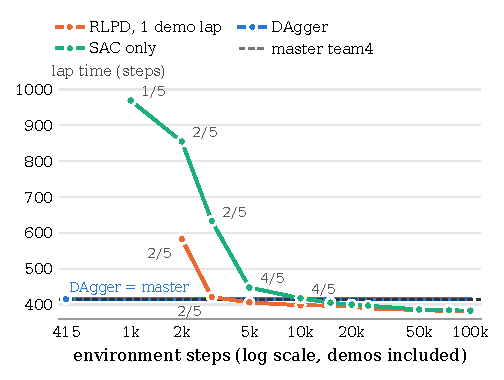
\includegraphics[width=\columnwidth]{fig1_learning.pdf}
\caption{\textbf{Training track (lighthouse).} Lap time of the evaluation episode vs environment steps; point = median lap time of the seeds that finish at this checkpoint, $k/5$ = number of seeds that finish when not all do. DAgger matches the master (dotted line) from the demo on. RLPD and SAC only reach their first lap at the same time (median 2000 steps, $p=0.88$), but RLPD reaches the master's lap time sooner (median 4500 vs 15000 steps, $p=0.016$); both end at 381 vs 383 steps.}
\label{fig:learning}
\end{figure}

\Cref{fig:learning} compares RLPD (one demo lap) with SAC only.
The demos do not help to find the finish line sooner: the first lap comes at the same time.
They make the agent reach the master's speed about three times sooner, and the mean lap time over the first 10k steps is lower (704 vs 915 steps, unfinished counted 1500, $p=0.07$).
After a long training there is no big difference (381 vs 383 steps), so \textbf{the speed of learning is the main gain of symmetric sampling} here.
Both end 8\% faster than the master: this comes from RL, not from the demos (the master is also limited by $\mathrm{Box}(2)$).
On the test tracks RLPD finishes more often than SAC only (0.25 vs 0.06, $p=0.032$), but both are far below DAgger.

\subsection{Generalisation: DAgger vs RLPD}

\begin{figure*}[t]
\centering
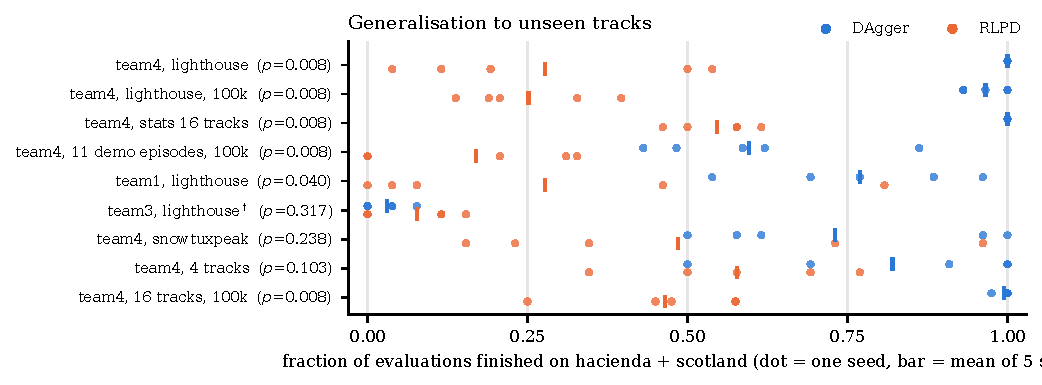
\includegraphics[width=\textwidth]{fig2_generalisation.pdf}
\caption{\textbf{Test tracks (hacienda + scotland), never seen in training.} For each setting (master, training tracks, demos), DAgger and RLPD get the same demos and normalisation statistics. Dot = fraction of evaluations finished from 5000 steps on, for one seed; bar = mean over 5 seeds; $p$ = exact two-sided permutation test on the means. Runs are compared up to 20k steps unless ``100k''. DAgger is better in 8 of 9 settings, significantly in 5. $^\dagger$team3 drifts 40\% of the time, which is lost in $\mathrm{Box}(2)$: both methods almost always fail.}
\label{fig:gen}
\end{figure*}

\Cref{fig:gen} gives the main result: \textbf{DAgger generalises much better than RLPD}.
With team4 on lighthouse, DAgger finishes almost every test evaluation while RLPD finishes about one in four ($p=0.008$, the smallest possible value).
On the training track it is the opposite: RLPD is faster than the master (381 vs 415 steps), DAgger equals it. But RLPD drives far from the centre of the track (3.3\,m vs 0.74\,m) with a jerky steering (0.21 vs 0.07): it \textbf{optimises a trajectory specific to the track}, while \textbf{DAgger copies a policy that transfers}.
More training tracks help RLPD (0.25 with 1 track, 0.58 with 4, 0.47 with 16) without closing the gap (DAgger 0.82 and 0.99).
The normalisation statistics matter for RLPD (0.55 with statistics on 16 tracks vs 0.25) but not for DAgger (1.00 in both cases).
Eleven times more demos (the clean lap + 10 noisy episodes) do not help RLPD: it reaches the master's lap time later (7500 vs 4500 steps, $p=0.024$) and does not generalise better.
With team3, both fail, which we attribute to the drift lost by the truncation.

\subsection{Why DAgger is behaviour cloning here}

\begin{table}[t]
\centering\small
\setlength{\tabcolsep}{3pt}
\caption{\textbf{DAgger loop on hacienda (test).} Seeds finishing at the BC point (before any iteration) $\to$ at the last point (20k steps), and finished evaluations from 5000 steps on. Without noise the loop never helps; executed-action noise $\sigma$ (labels stay clean) makes it useful again.}
\label{tab:loop}
\resizebox{\columnwidth}{!}{\begin{tabular}{lcc}
\toprule
setting & BC $\to$ end & evals $\geq$5k \\
\midrule
team4, lighthouse & 5 $\to$ 5 & 65/65 \\
team1, lighthouse & 5 $\to$ 2 & 35/65 \\
team4, 8 tracks & 5 $\to$ 3 & 52/61 \\
team4, snowtuxpeak & 5 $\to$ 1 & 30/65 \\
\quad + noise $\sigma=0.1$ / $0.3$ & 5 $\to$ 5 / 5 $\to$ 5 & 45/64 \,/\, 56/65 \\
team4, 11 demo episodes (executed actions) & 5 $\to$ 1 & 33/65 \\
\quad same, relabelled by the master & 5 $\to$ 5 & 65/65 \\
\bottomrule
\end{tabular}}
\end{table}

The environment is deterministic and the student equals the master from the demo on: each DAgger iteration replays the same lap (415 steps on lighthouse) and the final dataset is about 48 copies of the same trajectory.
The loop has no error state to correct, so what we measure is the generalisation of behaviour cloning, and \textbf{100k steps bring nothing more than 20k}.
\Cref{tab:loop} shows that without noise the loop never improves generalisation and sometimes degrades it (cause not established; possibly overfitting with 200 gradient steps per iteration on nearly duplicated data).
When noise is added to the executed action, the student visits states off the master's trajectory and the loop helps again (snowtuxpeak: 1 $\to$ 5 seeds); it is not always positive (team1 with $\sigma=0.3$: 0/5).
The noisy demos given to RLPD store the executed action (master + noise): for DAgger these are biased labels, and relabelling them with the master restores 65/65.

\subsection{Cost}
A DAgger run of 20k steps takes about 10\,min (local machine); an RLPD run of 100k steps about 3.5\,h (Kaggle, 2 threads) and about 5.8\,h locally (5 runs in parallel, 1 thread each, machine partly shared with other jobs). The machines differ, but RLPD costs 10 to 20 times more compute for the same number of environment steps (UTD 4 and the critics).

\section{Discussion}
\label{sec:discussion}

\paragraph{Information is not the same.}
An equal budget in environment steps is not equal information: DAgger queries the master at every step (20k to 100k labels), RLPD only has the demos and the reward.
This is why \textbf{DAgger needs a master that is available at training time}, while \textbf{RLPD only needs a dataset} and can go beyond the master, which it does on the training track.
In our setting the master's policy is a smooth function of the observation, so copying it transfers well; RLPD optimises the reward of one track and overfits it.

\paragraph{Limits.}
The environment and the evaluations are deterministic (1 episode per evaluation), so our 5 seeds only measure training variability, and 5 vs 5 tests have little power (the non-significant settings are not evidence of equality).
Our RLPD is simplified (2 critics, UTD 4, state-independent $\log\sigma$, no hyperparameter search).
The truncated actions limit the masters (no drift, no nitro), which hurts team3 most.
The RLPD settings were chosen after reading the DAgger results, test tracks included: this is a choice of comparison, not tuning, but it is a risk.
Finally, everything is single-kart; the competition setting with opponents was not tested.

{\small
\bibliographystyle{plain}
\bibliography{references}
}

\end{document}
